\section{Results}\label{sec:results}
\subsection{Proving and Verifying Times}\label{subsec:results:provingverifying}

\begin{figure*}[!htb]
    \centering
    \subfloat[\centering Proving Time]{{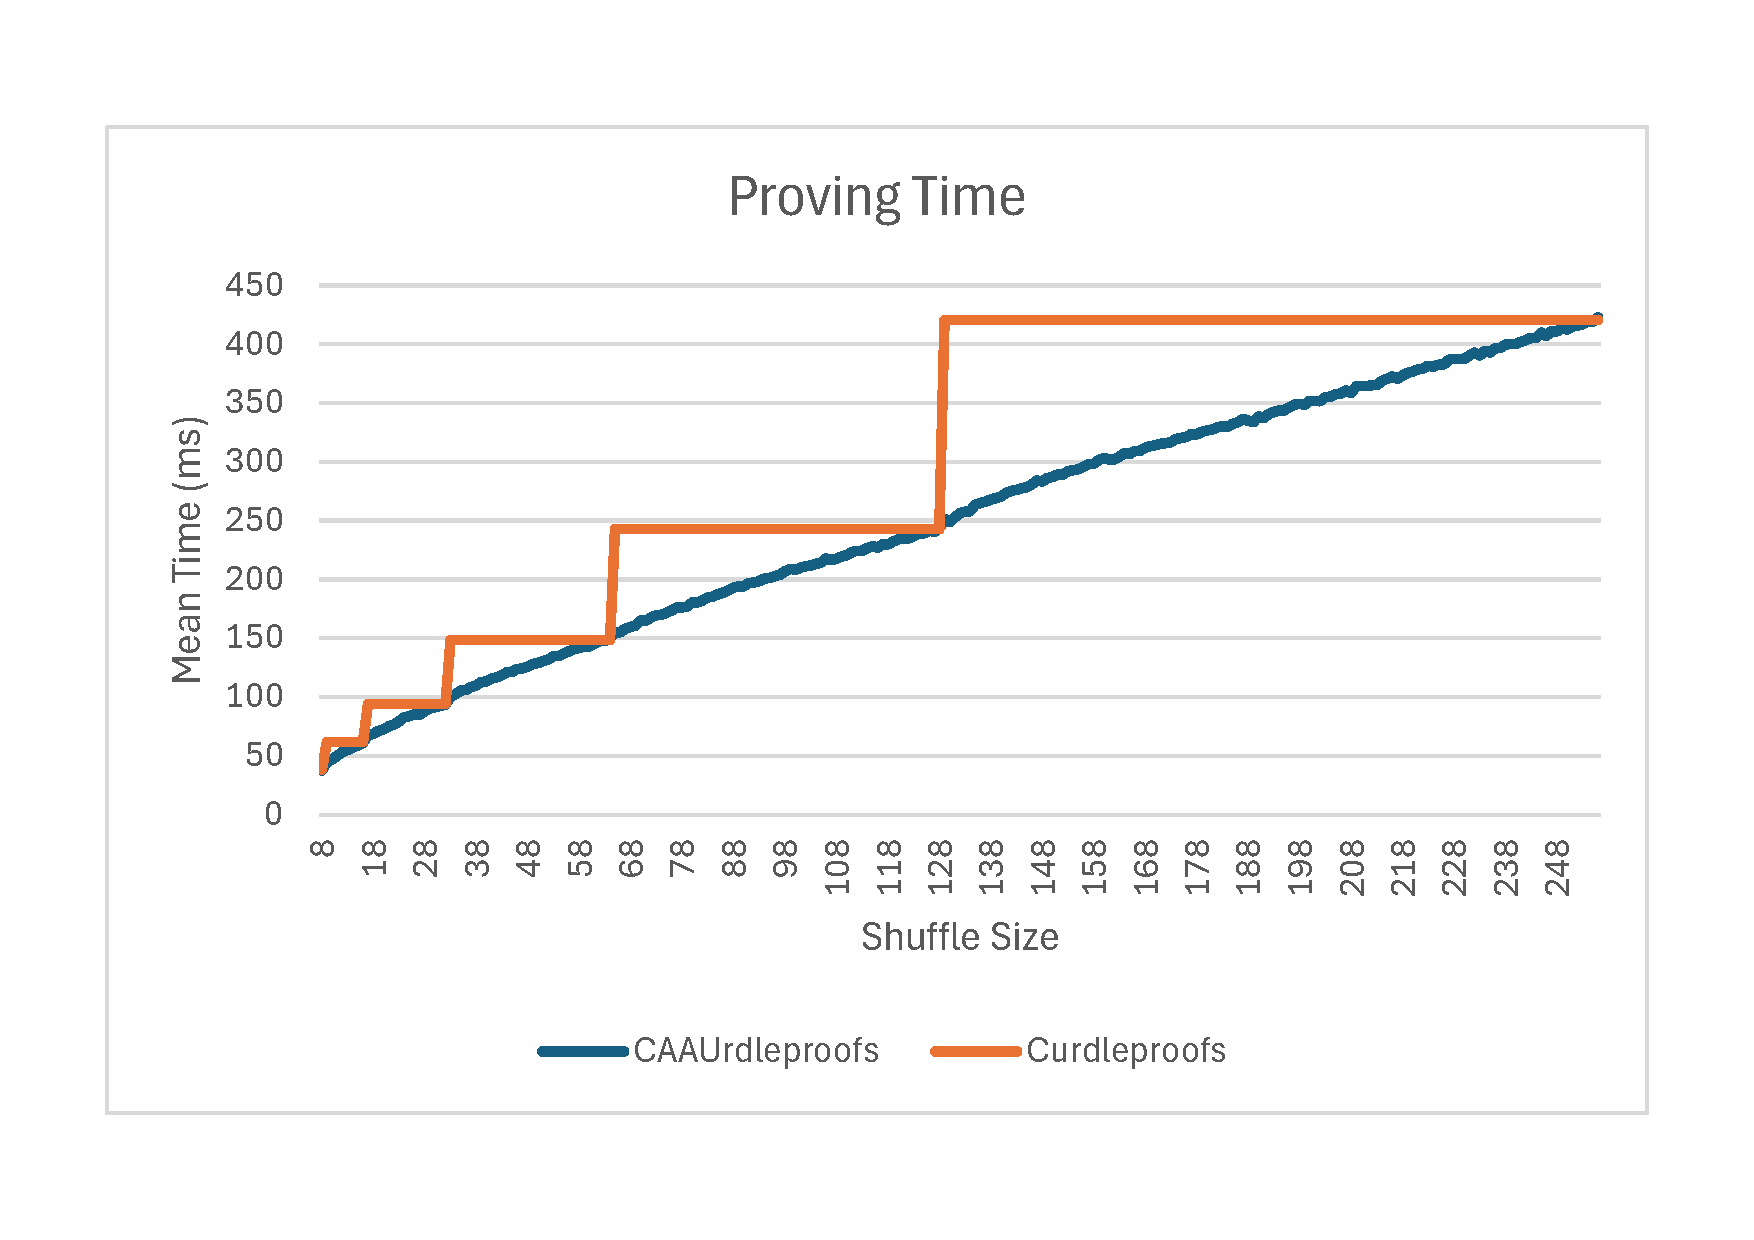
\includegraphics[width=0.45\textwidth]{figures/results/provingtime} }}%
    \qquad
    \subfloat[\centering Verifying Time]{{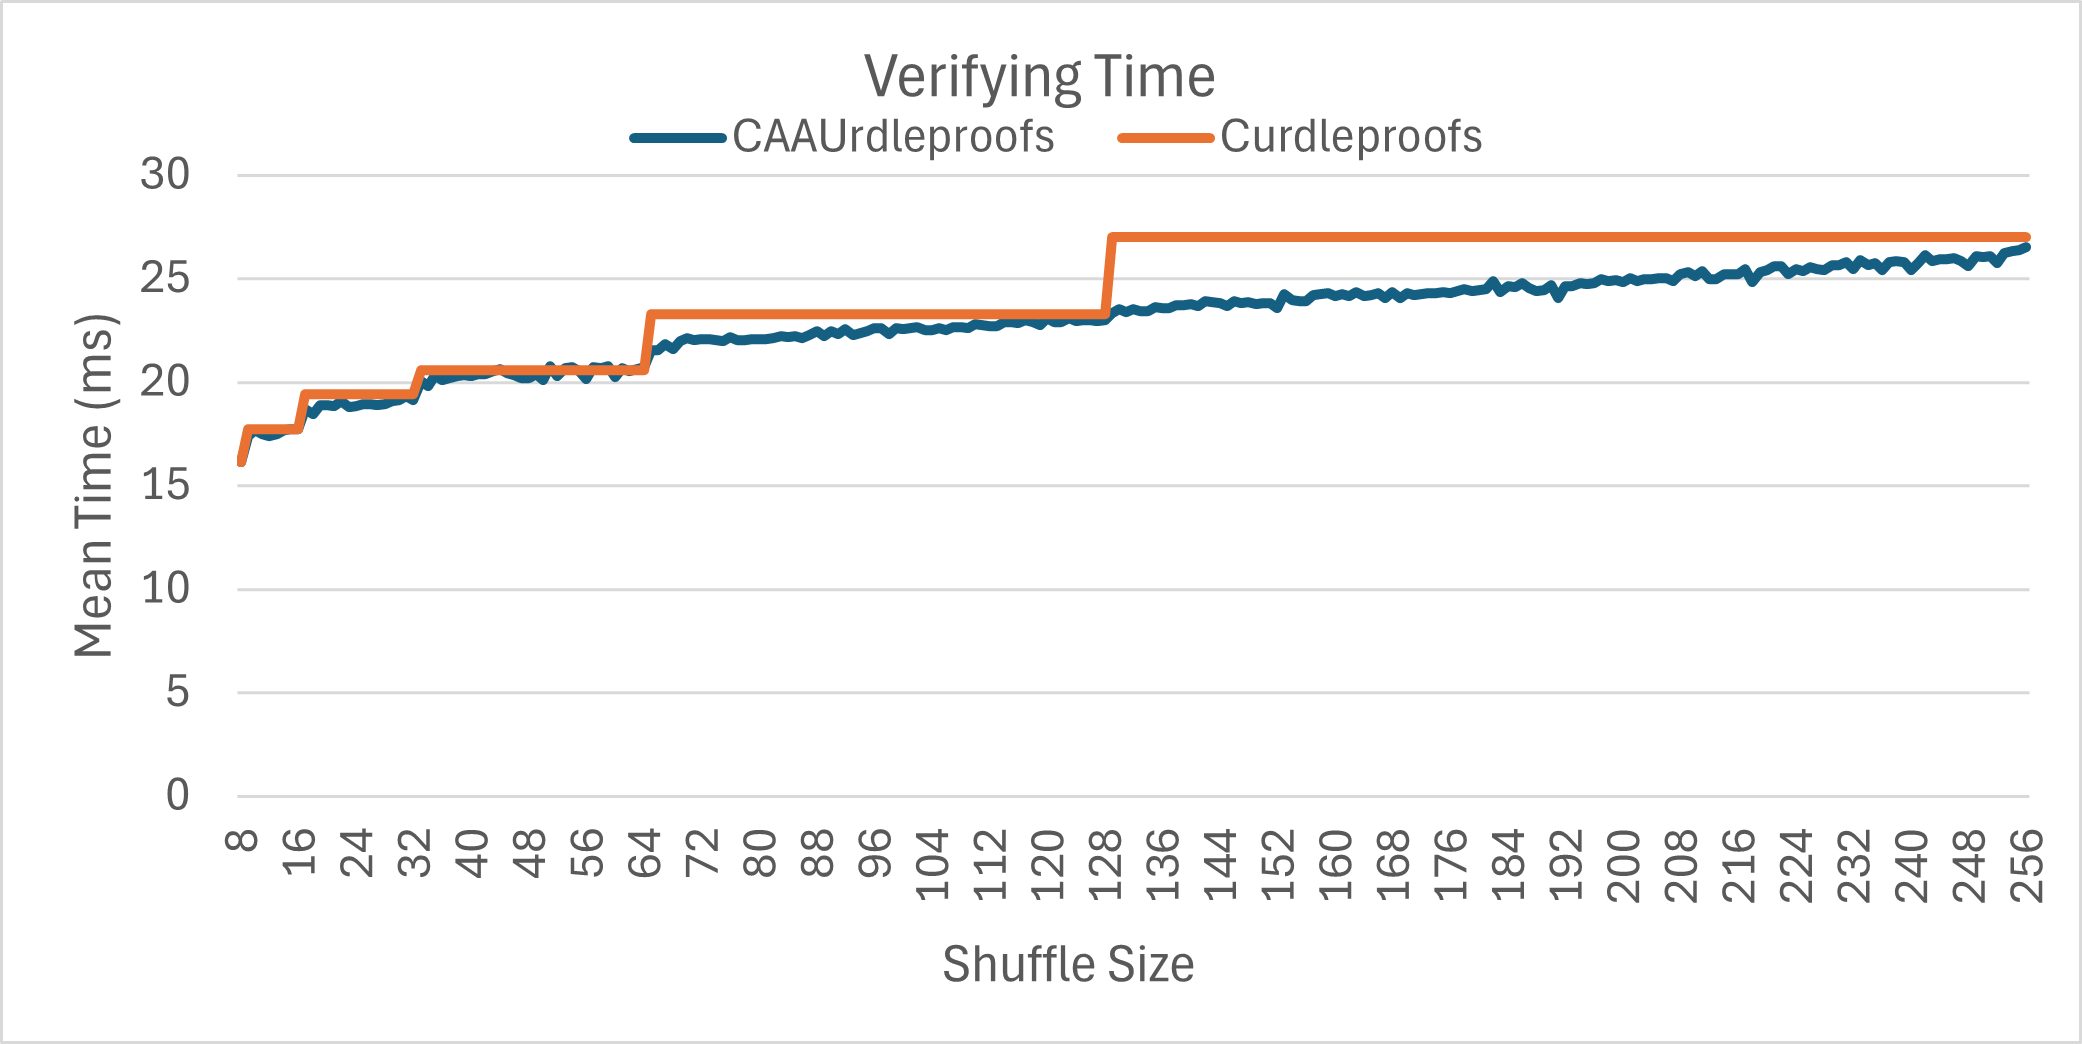
\includegraphics[width=0.45\textwidth]{figures/results/verifyingtime} }}%
    \caption{The timed results compared between CAAUrdleProofs and Curdleproofs}%
    \label{fig:resulttimes}%
\end{figure*}

After running the experiment where Curdleproofs and CAAUrdleproofs were compared across different shuffle sizes, we obtained the results shown in \autoref{fig:resulttimes}.

As mentioned in \autoref{sec:CAAUrdleproof-experiment}, CAAUdleproofs was run with a shuffle size $k$ of $\{8,9,\dots,256\}$ but Curdleproofs was only run with a shuffle size $k$ of $\{8,16,32,64,128,256\}$.
This is why the results for Curdleproofs show the shuffle size, $\ell$, instantly goes up to the next power of 2, because it theoretically would have to pad the input set until it reached the next power of 2.

From the results, we can see that CAAUrdleproofs and Curdleproofs have similar proving and verifying times when $\ell$ is a power of 2.
However, when $k$ is not a power of 2, CAAUrdleproofs is faster.

Additional to the proving and verifying times, the time used on shuffling is also lower for any $k$ that is not a power of 2, but that was to be expected since CAAUrdleproofs uses the same shuffling algorithm but does not have to add additional padding values to the non power of 2 input sizes.


\subsection{Shuffle security}\label{subsec:Shuffle-security}

\begin{figure*}[!htb]
    \centering
    \subfloat[\centering]{{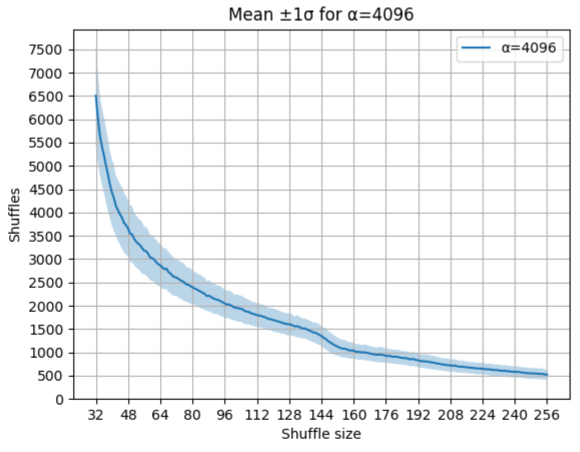
\includegraphics[width=0.45\textwidth]{figures/results/4096-256-p2} }}%
    \qquad
    \subfloat[\centering]{{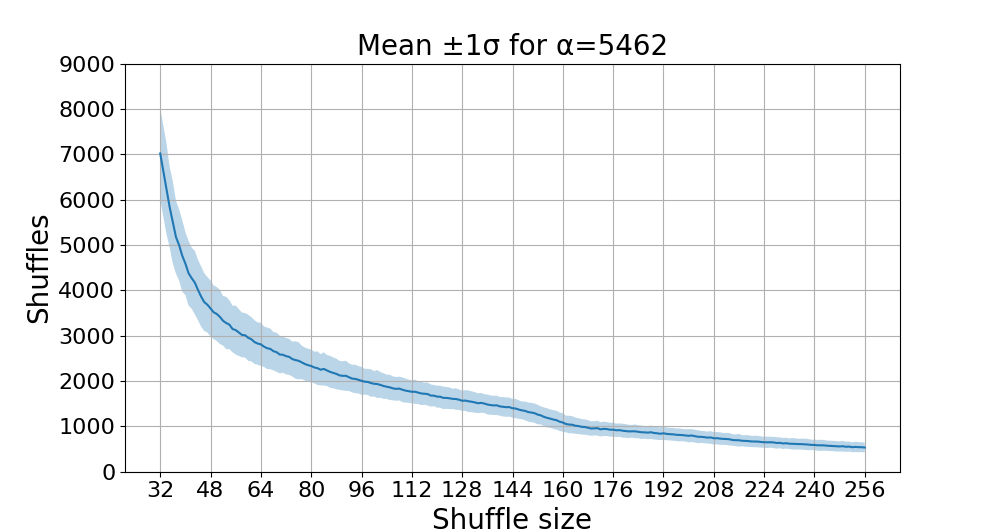
\includegraphics[width=0.45\textwidth]{figures/results/5462-256-p2} }}%
    \subfloat[\centering]{{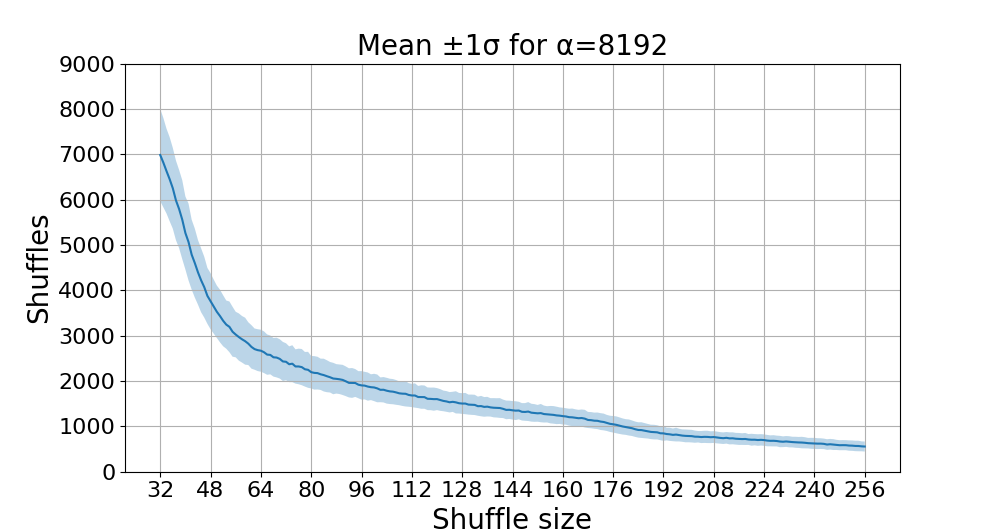
\includegraphics[width=0.45\textwidth]{figures/results/8192-256-p2} }}%
    \caption{The results of the shuffle security experiment showing the mean amount of honest shuffles necessary with one standard deviation}%
    \label{fig:shufflesecurity}%
\end{figure*}

The results of the shuffle security experiment are shown in \autoref{fig:shufflesecurity}.

\autoref{fig:shufflesecurity} shows the mean of the 1000 runs of each shuffle size $k$ as well as one standard deviation higher and lower.

We can see that the bigger the shuffle size $k$ the less honest shuffles are necessary to make the shuffle secure.
We also see that the bigger the shuffle size the smaller the deviation is between necessary honest shuffles become.

From the results of the experiment with $\alpha=8192$ we can see that number of honest shuffles necessary to make the shuffle secure sharply goes down until a size of $k=64$, and then it starts to flatten out.
we can see that with a size of $k=75$ we need about 1/3 of the shuffles to be honest to make the shuffle secure.
Likewise, we can see the at $k=108$ we need about 1/4 of the shuffles to be honest to make the shuffle secure.

In general all three of the experiments despite the difference in $\alpha$ show the same trend.
There are two things however that are different between the experiments.
At an $\alpha$ of 4096 we can see that the mean number of honest shuffles necessary to make the shuffle secure is 500 lower than the 2 others.
Another thing that differs between the experiments is that they all have sudden dip later on in the experiment.
Here we can see a trend that the lower the~$\alpha$ the earlier the dip happens.